\section{Related Work}
\label{sec:related-work}
% \textbf{Explainable Artificial Intelligence on Time-Series Data} An Overview of existing Explainable Artificial Intelligence (XAI) on Time-Series Data shows that the main focus is on the classification task.

% We are interested in post-hoc explainability methods, with a preference for model-agnostic types. Post-hoc methods refer to the fact that the explainability module wraps the model to produce an explanation. On the other hand, ante-hoc methods incorporate the explainability module into the model's architecture. The agnostic type refers to the fact that the explainability methods do not depend on the model and should work with any type of model. 

% The scope of the explanation can be either local or global. The local scope would mean that the methods could explain which behaviours for the patient are good or bad. General scope tends to identify good or bad behaviour in the whole population.

% The target of the explanation is the patient himself.

% And the problem type should be extrinsic regression.
% 
\begin{table*}[h!]
  \centering
  \begin{tabular}{@{}ccccccccccc@{}}
    \toprule
    Date        &   Authors                         & Model             & Methods       & Spec./Agno.   & Scope         & Target  & Problem Type                      & Citations         & Code \\
    \midrule

    2013        & Senin\cite{senin_sax-vsm_2013}             &\textit{Sax-vsm}   & SAX           & Specific      & Global        & Dev.      & Classification                    & 379               & \href{https://github.com/jMotif/sax-vsm_classic}{code}\\ 
    
    2016        &   Wang \cite{wang_time_2016}        & \textit{FCN}      & Backprop.     & Specific      & Local         & Dev.      & Classification                    & 1688              & \href{https://github.com/cauchyturing/UCR_Time_Series_Classification_Deep_Learning_Baseline}{code}\\ 

    2017        & Karim\cite{karim_multivariate_2019}             &\textit{\footnotesize{LSTM-FCN}} & Attention     &Specific       & Local         & Dev.      & Classification                    & 1143              & \href{https://github.com/houshd/LSTM-FCN}{code}\\ 

    2018        & Wachter\cite{wachter_counterfactual_2018} & \textit{W-CF} & CF    & Agnostic      & Local         & User      & Classification & 2584 & \href{https://github.com/e-delaney/Instance-Based_CFE_TSC/tree/main/W-CF}{code}\\

    2018        & Vinayavekhin\cite{vinayavekhin_focusing_2018} &\textit{TCL}& Attention &Specific        & Local         & Dev.      & Class. \& Fore.                           & 25                & no\\  

    2018        & Strodthoff\cite{strodthoff_detecting_2019}  &\textit{\footnotesize{MI-FCNN}}   & Backprop.     &Specific       & Local         & User   & Classification                    & 176               & no\\ 

    2018        & Siddiqui\cite{siddiqui_tsviz_2019}       &\textit{Tsviz}     & Backprop.     &Specific       & Both          & Dev.      & Class. \& Reg.                    & 78                & \href{https://github.com/shoaibahmed/TSViz-Core}{code}\\

    2018        & Le Nguyen\cite{nguyen_interpretable_2018}&\textit{SEQL}&SAX        &Specific       & Global        & Dev.      & Classification                    & 11                & \href{https://github.com/lnthach/Mr-SEQL}{code}\\ 

    2018        & Cho\cite{cho_interpretation_2020}   &\textit{CHAP}      & Backprop.     & Specific      & Both          & Dev.      & Classification                           & 176               & no\\

    2018        & Ge\cite{ge_interpretable_2018}      &\textit{\footnotesize{ICU-LSTM}}  & Attention     &Specific       & Global        & Dev.      & Prediction                        & 68                & no \\  

    2018        & El-Sappagh\cite{el-sappagh_ontology-based_2018}   & \textit{FAHP}     & Fuzy logic    &Specific       & Global        & User      & Classification                    & 78                & no\\ 

    2019        &   Fawaz \cite{ismail_fawaz_accurate_2019}  & \textit{\footnotesize{ESS-CNN}}  & Backprop.     &Specific       & Local         & User   & Class. \& Reg.                    & 86                & \href{https://github.com/hfawaz/ijcars19}{code}\\ 

    2019        &  Wang\cite{wang_learning_2019}      &\textit{PR-CNN} & Sapelets      &Specific       & Global        & Dev.      & Classification                    & 17                & no\\ 

    2019        &   Oviedo \cite{oviedo_fast_2019}    & \textit{AutoXRD}  & Backprop.     &Specific       & Both          & Dev.      & Classification                    & 198               & \href{https://github.com/PV-Lab/autoXRD/tree/master}{code}\\ 

    2019        & Kashiparekh\cite{kashiparekh_convtimenet_2019}&\textit{ConvNet}& Perturbation  &Agnostic       & Local         & Dev.      & Classification                    & 89                & no \\ 

    2019        & Choi\cite{choi_fully_2021}               &\textit{IDH}& Attention   &Specific       & Local         & Dev.      & Classification                                 & 92                & \href{https://github.com/yoonchoi-neuro/automated_hybrid_IDH}{code}\\  

    2019        & Tonekaboni\cite{tonekaboni_explaining_2019}&\textit{FFC}& CF&Agnostic    & Both          & Dev.      & Classification                           & 8                & no \\ 

    2019        & Assaf\cite{assaf_mtex-cnn_2019}                  &\textit{Mtex-cnn}  & Backprop.&Specific       & Local         & Dev.      & Forecasting                        & 51                & no\\ 

    2019        & Munir\cite{munir_tsxplain_2019}            &\textit{Tsxplain}  &  Backprop.    &Agnostic       & Local         & Dev.      & Classification                    & 17                & no\\  

    2019        & Gee\cite{gee_explaining_2019}        &\textit{PDL}       & Prototypes    &Specific       & Global        & Dev.      & Classification                    & 66                & \href{https://github.com/alangee/ijcai19-ts-prototypes}{code} \\ 

    2020        & Li\cite{li_efficient_2022}                   &\textit{\footnotesize{BSPCOVER}}  & Shapelets     & Specific      & Global        & Dev.      & Classification                    & 43               & no\\  

    2020        & Augustin\cite{augustin_adversarial_2020}&\textit{RATIO} & CF&Agnostic      & Local         & Dev.      & Training                          & 70                & \href{https://github.com/M4xim4l/InNOutRobustness}{code}\\ 
    
    2020        & Hao\cite{hao_new_2020}                 &\textit{CA-SFCN}   & Attention     &Specific       & Local         & Dev.      & Classification                    & 30                & \href{https://github.com/huipingcao/nmsu_yhao_ijcai2020}{code}\\ 

    2020        &   Wolanin\cite{wolanin_estimating_2020}       & \textit{CY-EDL}   & Backprop.     &Specific       & Both          & User   & Forecasting                          & 125               & no \\

    2020        & Kidger\cite{kidger_generalised_2020}& \textit{GST}      & Shapelets     &Specific       & Global        & Dev.      & Classification                    & 9                 & \href{https://github.com/patrick-kidger/generalised_shapelets}{code}\\  

    2020        & Schockaert\cite{schockaert_attention_2020} & \textit{\footnotesize{AM-LSTM}}& Attention&Specific       & Both          & Dev.      & Forecasting                       & 6                 & no\\ 

    2020        & Siddiqui\cite{siddiqui_tsinsight_2020}& \textit{Tsinsight}& Attention   &Specific       &Both           & Dev.      & Classification                    & 12                & no \\ 

    2020        & Tan\cite{tan_explainable_2021}                 &\textit{\footnotesize{eUA-CRNN}}  & Attention     &Specific       & Local         & Dev.      & Classification                                & 28                & no\\  

    2020        & Pan\cite{pan_series_2020}           &\textit{Saliency}& Perturbation    &Agnostic       & Local         & Dev.      & Forecasting                       & 7                 & no \\ 

    2020        & Ismail\cite{ismail_benchmarking_2020}           &\textit{Saliency}& Perturbation    &Agnostic       & Local         & Dev.      & Classification                    & 124               & \href{https://github.com/ayaabdelsalam91/TS-Interpretability-Benchmark}{code}\\ 

    2020        & Wang\cite{wang_deep_2021}           & \textit{\footnotesize{Deep-FCM}}& Fuzzy logic    &Specific       & Global        & Dev.      & Prediction                        & 39                & no\\ 

    2020        & Lauristsen\cite{lauritsen_early_2020}   &\textit{TCN}       &Backprop.      &Specific       & Both          & Dev.      & Classification                    & 234               & \href{https://github.com/albermax/innvestigate}{1} and \href{https://github.com/slundberg/shap}{2} \\

    2021        &Crabbé\cite{crabbe_explaining_2021}    & \textit{DynaMask}     & Perturbation  & Agnostic      & Local     & Dev.      & Class. \& Reg.                    & 55            & \href{https://github.com/JonathanCrabbe/Dynamask}{code}   \\ 

    2021        & Lim\cite{lim_temporal_2020}         & \textit{TFT}      & Attention     &Specific       & Both          & Dev.      & Forecasting                       & 822               & \href{https://github.com/greatwhiz/tft_tf2}{code}       \\ 

    2021        & Delaney\cite{delaney_instance-based_2021} & \textit{\footnotesize{Native Guide}} & CF & Agnostic & Local & Both      & Classification & 92 & \href{https://github.com/e-delaney/Instance-Based_CFE_TSC/tree/main}{code} \\
  
    2022        &Gao\cite{gao_explainable_2022}       &  \textit{ETNODE}  & Attention     &Specific       & Both          & Dev.      & Forecasting                        & 8                 & \href{https://github.com/PengleiGao/ETN-ODE}{code} \\  

    2023        &Zhao\cite{zhao_explainable_2023}                &\textit{Att-TCN}   & Perturbation             & Agnostic             & Both             & Dev.          & Classification                    & 3                 & no \\ 

    2023        & Höllig\cite{hollig_tsevo_2022}           & \textit{TSEvo}& CF           & Agnostic             & Local             & User         & Classification                                 & 5                 & \href{https://github.com/fzi-forschungszentrum-informatik/TSInterpret}{code} \\

    2024        & Ours           & \textit{TSEvoR}& CF           & Agnostic             & Local             & User         & Regression                   & -                 & \href{https://github.com/AlexisTabin/BA-Estimation-TCN}{code} \\

    \bottomrule
  \end{tabular}
  \caption{Comparison of the existing XAI techniques for Time-Series, adapted from \cite{rojat_explainable_2021}}
\end{table*}

% \textbf{Counterfactuals Explanations for Time-Series Classification} Counterfactuals are very close to Adversarial Perturbations \cite{moosavi-dezfooli_universal_2017}. The main difference between them is the sparsity factor. Adversarial Perturbations are used mainly when handling image classification. The goal is to show that a very similar image could be classified differently with changes in the input that are unnoticeable by the human eye. To achieve that, the Adversarial Perturbation model modifies many variables by a small value, whereas the Counterfactuals want to modify the least number possible of variables to achieve human interpretable solutions. Wachter \& Al. \cite{wachter_counterfactual_2018} were among the first to propose a Counterfactual theory. 
% Definition of Counterfactuals, Wachter equation 

% \textbf{GAP - From Counterfactuals for Time-Series Classification to Counterfactuals for Time-Series Extrinsic Regression}
% Explain existing techniques

%============ Written by ChatGPT ============
\subsection{Explainable Artificial Intelligence on Time-Series Data} Existing research on Explainable Artificial Intelligence (XAI) for time-series data predominantly focuses on classification tasks. \\
Here, the emphasis will be put on post-hoc explainability methods, specifically prioritizing techniques that work across different types of models, known as model-agnostic approaches.
Post-hoc methods wrap an explainability module around the model to generate explanations, contrasting with ante-hoc methods that integrate explainability within the model's architecture.
Model-agnostic methods are preferred due to their versatility across various model types. \\
Additionally, explainability scopes vary, encompassing both local and global perspectives.
Local explanations provide insights into individual behaviours, while global explanations discern broader trends within populations.
Crucially, the patients themselves are the target audience for explanations, aligning with the overarching goal of personalized healthcare interventions.\\
Furthermore, the problem type addressed typically falls under the name of time-series extrinsic regression, where the goal is to learn a relationship between a time-serie and a continuous scalar variable \cite{tan_time_2021}.


\begin{table*}[h!]
  \centering
  \begin{tabular}{@{}ccccccccccc@{}}
    \toprule
    Date        &   Authors                         & Model             & Methods       & Spec./Agno.   & Scope         & Target  & Problem Type                      & Citations         & Code \\
    \midrule

    2013        & Senin\cite{senin_sax-vsm_2013}             &\textit{Sax-vsm}   & SAX           & Specific      & Global        & Dev.      & Classification                    & 379               & \href{https://github.com/jMotif/sax-vsm_classic}{code}\\ 
    
    2016        &   Wang \cite{wang_time_2016}        & \textit{FCN}      & Backprop.     & Specific      & Local         & Dev.      & Classification                    & 1688              & \href{https://github.com/cauchyturing/UCR_Time_Series_Classification_Deep_Learning_Baseline}{code}\\ 

    2017        & Karim\cite{karim_multivariate_2019}             &\textit{\footnotesize{LSTM-FCN}} & Attention     &Specific       & Local         & Dev.      & Classification                    & 1143              & \href{https://github.com/houshd/LSTM-FCN}{code}\\ 

    2018        & Wachter\cite{wachter_counterfactual_2018} & \textit{W-CF} & CF    & Agnostic      & Local         & User      & Classification & 2584 & \href{https://github.com/e-delaney/Instance-Based_CFE_TSC/tree/main/W-CF}{code}\\

    2018        & Vinayavekhin\cite{vinayavekhin_focusing_2018} &\textit{TCL}& Attention &Specific        & Local         & Dev.      & Class. \& Fore.                           & 25                & no\\  

    2018        & Strodthoff\cite{strodthoff_detecting_2019}  &\textit{\footnotesize{MI-FCNN}}   & Backprop.     &Specific       & Local         & User   & Classification                    & 176               & no\\ 

    2018        & Siddiqui\cite{siddiqui_tsviz_2019}       &\textit{Tsviz}     & Backprop.     &Specific       & Both          & Dev.      & Class. \& Reg.                    & 78                & \href{https://github.com/shoaibahmed/TSViz-Core}{code}\\

    2018        & Le Nguyen\cite{nguyen_interpretable_2018}&\textit{SEQL}&SAX        &Specific       & Global        & Dev.      & Classification                    & 11                & \href{https://github.com/lnthach/Mr-SEQL}{code}\\ 

    2018        & Cho\cite{cho_interpretation_2020}   &\textit{CHAP}      & Backprop.     & Specific      & Both          & Dev.      & Classification                           & 176               & no\\

    2018        & Ge\cite{ge_interpretable_2018}      &\textit{\footnotesize{ICU-LSTM}}  & Attention     &Specific       & Global        & Dev.      & Prediction                        & 68                & no \\  

    2018        & El-Sappagh\cite{el-sappagh_ontology-based_2018}   & \textit{FAHP}     & Fuzy logic    &Specific       & Global        & User      & Classification                    & 78                & no\\ 

    2019        &   Fawaz \cite{ismail_fawaz_accurate_2019}  & \textit{\footnotesize{ESS-CNN}}  & Backprop.     &Specific       & Local         & User   & Class. \& Reg.                    & 86                & \href{https://github.com/hfawaz/ijcars19}{code}\\ 

    2019        &  Wang\cite{wang_learning_2019}      &\textit{PR-CNN} & Sapelets      &Specific       & Global        & Dev.      & Classification                    & 17                & no\\ 

    2019        &   Oviedo \cite{oviedo_fast_2019}    & \textit{AutoXRD}  & Backprop.     &Specific       & Both          & Dev.      & Classification                    & 198               & \href{https://github.com/PV-Lab/autoXRD/tree/master}{code}\\ 

    2019        & Kashiparekh\cite{kashiparekh_convtimenet_2019}&\textit{ConvNet}& Perturbation  &Agnostic       & Local         & Dev.      & Classification                    & 89                & no \\ 

    2019        & Choi\cite{choi_fully_2021}               &\textit{IDH}& Attention   &Specific       & Local         & Dev.      & Classification                                 & 92                & \href{https://github.com/yoonchoi-neuro/automated_hybrid_IDH}{code}\\  

    2019        & Tonekaboni\cite{tonekaboni_explaining_2019}&\textit{FFC}& CF&Agnostic    & Both          & Dev.      & Classification                           & 8                & no \\ 

    2019        & Assaf\cite{assaf_mtex-cnn_2019}                  &\textit{Mtex-cnn}  & Backprop.&Specific       & Local         & Dev.      & Forecasting                        & 51                & no\\ 

    2019        & Munir\cite{munir_tsxplain_2019}            &\textit{Tsxplain}  &  Backprop.    &Agnostic       & Local         & Dev.      & Classification                    & 17                & no\\  

    2019        & Gee\cite{gee_explaining_2019}        &\textit{PDL}       & Prototypes    &Specific       & Global        & Dev.      & Classification                    & 66                & \href{https://github.com/alangee/ijcai19-ts-prototypes}{code} \\ 

    2020        & Li\cite{li_efficient_2022}                   &\textit{\footnotesize{BSPCOVER}}  & Shapelets     & Specific      & Global        & Dev.      & Classification                    & 43               & no\\  

    2020        & Augustin\cite{augustin_adversarial_2020}&\textit{RATIO} & CF&Agnostic      & Local         & Dev.      & Training                          & 70                & \href{https://github.com/M4xim4l/InNOutRobustness}{code}\\ 
    
    2020        & Hao\cite{hao_new_2020}                 &\textit{CA-SFCN}   & Attention     &Specific       & Local         & Dev.      & Classification                    & 30                & \href{https://github.com/huipingcao/nmsu_yhao_ijcai2020}{code}\\ 

    2020        &   Wolanin\cite{wolanin_estimating_2020}       & \textit{CY-EDL}   & Backprop.     &Specific       & Both          & User   & Forecasting                          & 125               & no \\

    2020        & Kidger\cite{kidger_generalised_2020}& \textit{GST}      & Shapelets     &Specific       & Global        & Dev.      & Classification                    & 9                 & \href{https://github.com/patrick-kidger/generalised_shapelets}{code}\\  

    2020        & Schockaert\cite{schockaert_attention_2020} & \textit{\footnotesize{AM-LSTM}}& Attention&Specific       & Both          & Dev.      & Forecasting                       & 6                 & no\\ 

    2020        & Siddiqui\cite{siddiqui_tsinsight_2020}& \textit{Tsinsight}& Attention   &Specific       &Both           & Dev.      & Classification                    & 12                & no \\ 

    2020        & Tan\cite{tan_explainable_2021}                 &\textit{\footnotesize{eUA-CRNN}}  & Attention     &Specific       & Local         & Dev.      & Classification                                & 28                & no\\  

    2020        & Pan\cite{pan_series_2020}           &\textit{Saliency}& Perturbation    &Agnostic       & Local         & Dev.      & Forecasting                       & 7                 & no \\ 

    2020        & Ismail\cite{ismail_benchmarking_2020}           &\textit{Saliency}& Perturbation    &Agnostic       & Local         & Dev.      & Classification                    & 124               & \href{https://github.com/ayaabdelsalam91/TS-Interpretability-Benchmark}{code}\\ 

    2020        & Wang\cite{wang_deep_2021}           & \textit{\footnotesize{Deep-FCM}}& Fuzzy logic    &Specific       & Global        & Dev.      & Prediction                        & 39                & no\\ 

    2020        & Lauristsen\cite{lauritsen_early_2020}   &\textit{TCN}       &Backprop.      &Specific       & Both          & Dev.      & Classification                    & 234               & \href{https://github.com/albermax/innvestigate}{1} and \href{https://github.com/slundberg/shap}{2} \\

    2021        &Crabbé\cite{crabbe_explaining_2021}    & \textit{DynaMask}     & Perturbation  & Agnostic      & Local     & Dev.      & Class. \& Reg.                    & 55            & \href{https://github.com/JonathanCrabbe/Dynamask}{code}   \\ 

    2021        & Lim\cite{lim_temporal_2020}         & \textit{TFT}      & Attention     &Specific       & Both          & Dev.      & Forecasting                       & 822               & \href{https://github.com/greatwhiz/tft_tf2}{code}       \\ 

    2021        & Delaney\cite{delaney_instance-based_2021} & \textit{\footnotesize{Native Guide}} & CF & Agnostic & Local & Both      & Classification & 92 & \href{https://github.com/e-delaney/Instance-Based_CFE_TSC/tree/main}{code} \\
  
    2022        &Gao\cite{gao_explainable_2022}       &  \textit{ETNODE}  & Attention     &Specific       & Both          & Dev.      & Forecasting                        & 8                 & \href{https://github.com/PengleiGao/ETN-ODE}{code} \\  

    2023        &Zhao\cite{zhao_explainable_2023}                &\textit{Att-TCN}   & Perturbation             & Agnostic             & Both             & Dev.          & Classification                    & 3                 & no \\ 

    2023        & Höllig\cite{hollig_tsevo_2022}           & \textit{TSEvo}& CF           & Agnostic             & Local             & User         & Classification                                 & 5                 & \href{https://github.com/fzi-forschungszentrum-informatik/TSInterpret}{code} \\

    2024        & Ours           & \textit{TSEvoR}& CF           & Agnostic             & Local             & User         & Regression                   & -                 & \href{https://github.com/AlexisTabin/BA-Estimation-TCN}{code} \\

    \bottomrule
  \end{tabular}
  \caption{Comparison of the existing XAI techniques for Time-Series, adapted from \cite{rojat_explainable_2021}}
\end{table*}

\subsection{Counterfactual Explanations for Time-Series Classification} Counterfactual explanations offer a compelling approach, differing from Adversarial Perturbations primarily in their emphasis on sparse modifications for human interpretability.
While Adversarial Perturbations focus on imperceptible changes to input data for image classification tasks, counterfactual methods strive to alter the fewest variables necessary to achieve interpretable solutions. \\


\subsubsection{Wachter} Pioneering work by Wachter et al. \cite{wachter_counterfactual_2018} laid the foundation for counterfactual theory, offering clear definitions and methodologies, including the influential Wachter equation.

%============ From Wachter paper ============
\begin{equation} \label{eq:1}
\arg \min _{w} \ell\left(f_{w}\left(x_{i}\right), y_{i}\right)+\rho(w)
\end{equation}

Where $y_{i}$ is the label for data point $x_{i}$ and $\rho(\cdot)$ is a regularizer over the weights. We wish to find a counterfactual $x^{\prime}$ as close to the original point $x_{i}$ as possible such that $f_{w}\left(x^{\prime}\right)$ is equal to a new target $y^{\prime}$. We can find $x^{\prime}$ by holding $w$ fixed and minimizing the related objective.


\begin{equation} \label{eq:2}
\arg \min _{x^{\prime}} \max _{\lambda} \lambda\left(f_{w}\left(x^{\prime}\right)-y^{\prime}\right)^{2}+d\left(x_{i}, x^{\prime}\right)
\end{equation}

Where $d(\cdot, \cdot)$ is a distance function that measures how far the counterfactual $x^{\prime}$ and the original data point $x_{i}$ are from one another. In practice, maximisation over $\lambda$ is done by iteratively solving for $x^{\prime}$ and increasing $\lambda$ until a sufficiently close solution is found.

The choice of optimiser for these problems is relatively unimportant. In practice, any optimiser capable of training the classifier under Equation 1 seems to work equally well, and we use $\mathrm{ADAM}$ \cite{kingma_adam_2017} for all experiments.
As local minima are a concern, we initialise each run with different random values for $x^{\prime}$ and select as our counterfactual the best minimizer of Equation 2. These different minima can be used as a diverse set of multiple counterfactuals.
%============ From Wachter paper ============
\subsubsection{Instance-Based}
% \documentclass[10pt]{article}
% \usepackage[utf8]{inputenc}
% \usepackage[T1]{fontenc}
% \usepackage{amsmath}
% \usepackage{amsfonts}
% \usepackage{amssymb}
% \usepackage[version=4]{mhchem}
% \usepackage{stmaryrd}
% \usepackage{bbold}
% \usepackage{graphicx}
% \usepackage[export]{adjustbox}
% \graphicspath{ {./images/} }
% \usepackage{hyperref}
% \hypersetup{colorlinks=true, linkcolor=blue, filecolor=magenta, urlcolor=cyan,}
% \urlstyle{same}

%New command to display footnote whose markers will always be hidden
\let\svthefootnote\thefootnote
\newcommand\blfootnotetext[1]{%
  \let\thefootnote\relax\footnote{#1}%
  \addtocounter{footnote}{-1}%
  \let\thefootnote\svthefootnote%
}

%Overriding the \footnotetext command to hide the marker if its value is `0`
\let\svfootnotetext\footnotetext
\renewcommand\footnotetext[2][?]{%
  \if\relax#1\relax%
    \ifnum\value{footnote}=0\blfootnotetext{#2}\else\svfootnotetext{#2}\fi%
  \else%
    \if?#1\ifnum\value{footnote}=0\blfootnotetext{#2}\else\svfootnotetext{#2}\fi%
    \else\svfootnotetext[#1]{#2}\fi%
  \fi
}

Like other case-based XAI methods $25,27,31,41$, at its core Native Guide relies upon existing instances in the training data, so-called native guides or nearest unlike neighbors (NUNs), that it retrieves and adapts to generate counterfactual explanations (see Figure 3). In this section, we outline the two main steps in the algorithm, after first describing the notation adopted.

\textbf{Notation.} Staying consistent with the notation of 15,18], a time series $T=\left\{\left\langle t_{1}, t_{2}, \ldots, t_{m}\right\rangle\right\}$ is an ordered set of real values, where $m$ is the length. A time series data set $\mathbf{T}=\left\{T_{1}, T_{2} \ldots, T_{n}\right\} \in \mathbb{R}^{n \times m}$ is a collection of such time series where each time series has a class label $c$ forming a vector of class labels $\mathbf{Y} \in \mathbb{Z}$. Consider a black-box classifier $b(T)$ that takes a time series $T$ as an input and predicts a probability output $P(\mathbf{Y} \mid T)$ over the label output space. Given a to-be-explained query time series $T_{q}$, with predicted label $c$ from the black-box classifier (formally $b\left(T_{q}\right)=c$ ), a counterfactual explanation aims to find how $T_{q}$ needs to change for the system to classify it alternatively, as $c^{\prime}$. We refer to $T^{\prime}$ as a counterfactual explanation for $T_{q}$ such that $b\left(T^{\prime}\right)=c^{\prime}$. Although there are many candidate solutions for $T^{\prime}$, the method prioritizes those that meet the four key properties of proximity, sparsity, plausibility and diversity.

\begin{figure}[h]
    \centering
    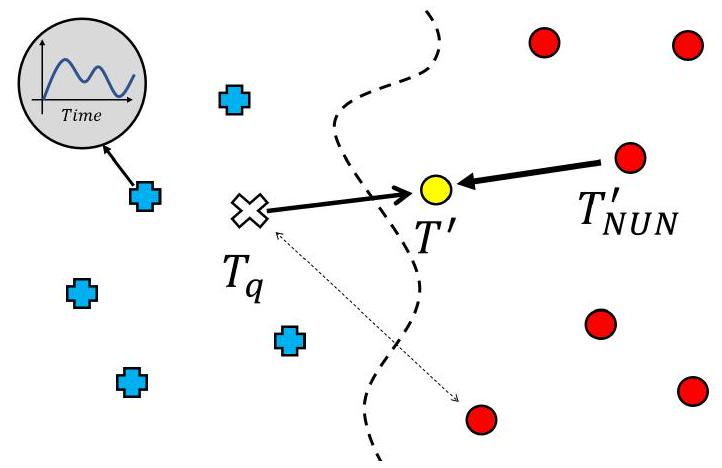
\includegraphics[width=0.4\textwidth]{CF/images/instance-based.jpg}
    \caption{A query time series $T_{q}$ (X with solid arrow) and a nearest-unlike neighbor, $T_{N U N}^{\prime}$ (red circle with solid arrow) are used to guide the generation of counterfactual $T^{\prime}$ (see yellow circle) in a binary classification task. Another in-sample counterfactual (i.e., the next NUN; other red circle with dashed arrow) could also be used to generate another counterfactual for diverse explanations.}
\end{figure}


\textbf{Step 1:} Retrieve native guide. Given a query time series, $T_{q}$, find a counterfactual instance, $T_{\text {Native }}^{\prime}$, that exists in the case-base. An example of one such instance is the query's nearest unlike neighbor $\left(T_{N U N}^{\prime}\right)$. In using these "native counterfactual" cases the method guarantees the explanation's plausibility as it is, by definition, within the distribution. However, such instances are not guaranteed to be sufficiently proximate to the query or, indeed, sparse, so an adaption step is necessary to generate the "explanatory counterfactual", $T^{\prime}$ (see Figure $3)$.

\textbf{Step 2:} Adapt native guide to generate counterfactual. To produce a more proximate explanatory counterfactual, $T^{\prime}$, the native guide, $T_{\text {Native }}^{\prime}$ is perturbed towards the to-be-explained query-case, $T_{q}$ (see Figure 3). Typically, counterfactual methods use some $L_{p}$ distance metric to guide this perturbation (such as Manhattan distance, [55]) and in time series where dynamic time warping (DTW) distance is often more appropriate an analogous averaging technique known as weighted dynamic barycentre averaging can be used 13]. In cases where we are explaining a deep-learner's predictions, the feature-weight vectors of the classifier, $\boldsymbol{\omega}$, can be used to perturb "semantically-meaningful" features of the time series, rather than the "raw" time series data, to guarantee sparsity ${ }^{4}$.
\footnotetext{Note, SHAP can also be used to generate such vectors, if we are directly explaining any given model, rather than twinning.
}

Accordingly, using the feature-weights, the method seeks to modify contiguous, subsequences, rather than the whole time series, as follows:

$$
\begin{aligned}
& T_{q}=\left\{<t_{1}, t_{2}, t_{3}, t_{4}, t_{5} \ldots, t_{n}>\right\} \text { s.t. } b\left(T_{q}\right)=c \\
& T^{\prime}=\left\{<t_{1}, t_{2}^{\prime}, t_{3}^{\prime}, t_{4}^{\prime}, t_{5} \ldots, t_{n}>\right\} \text { s.t. } b\left(T^{\prime}\right)=c^{\prime}
\end{aligned}
$$



\footnotetext{\href{https://github.com/e-delaney/Instance-Based_CFE_TSC}{https://github.com/e-delaney/Instance-Based\_CFE\_TSC}
}



%============ From TSEvo paper ============
\subsubsection{TSEvo}
We study a supervised time series classification problem. Let $x=\left[x_{1}, \ldots, x_{T}\right] \in \mathbb{R}^{N \times T}$ be a uni- or multivariate time series, where $T$ is the number of time steps and $N$ is the number of features. Let $x_{i, t}$ be the input feature $i$ at time $t$. Similarly, let $X_{:, t} \in R^{N}$ and $X_{i,:} \in R^{T}$ be the feature vector at time $t$, and the time vector for feature $i$, respectively. $Y$ denotes the output, and $f: x \rightarrow Y$ a classification model returning a probability distribution vector over classes $Y=\left[y_{1}, \ldots, y_{C}\right]$, where $C$ is the total number of classes (i.e., outputs) and $y_{i}$ the probability of $x$ belonging to class $i$. The classification model $f$ is seen as a "black-box" - i.e., no access to the inner workings of a model are available. Only the result $Y$ is observable.

\begin{definition}
Goal Properties of the TSEvo counterfactual search.
$$
\begin{aligned}
& \mathbf{R}_{\mathbf{1}}: \min \left(d\left(x, x^{c f}\right)\right), \text { s.t. } f(x) \neq f\left(x^{c f}\right) \\
& \mathbf{R}_{\mathbf{2}}: \min \left(\sum_{i=1}^{N} \sum_{t=1}^{T} \mathbbm{1}_{\left|x_{i, t}-x_{i, t}^{c f}\right| !=0}\right), \text { s.t. } f(x) \neq f\left(x^{c f}\right) \\
& \\
& \mathbf{R}_{\mathbf{3}}: x^{c f} \sim D, \text { s.t. } f(x) \neq f\left(x^{c f}\right)
\end{aligned}
$$ 
\end{definition}
The goal of counterfactual approaches is, given a time series $x$ and a classifier $f$, to provide an explanation via counter examples allowing humans to understand why classifier $f$ chose class $y$ for data point $x$ and not a counterfactual class $y^{c f}$ \cite{wachter_counterfactual_2018}. To allow such understanding, we assume that for each $x$, a counterfactual sample $x^{c f}$ can be computed, that is close to $x$, but differently classified $y \neq y^{c f}$. The resulting $x^{c f}$ is supposed to be a proximate $\left(\mathbf{R}_{1}\right)$ \cite{mothilal_explaining_2020}, sparse $\left(\mathbf{R}_{\mathbf{2}}\right)$ \cite{mothilal_explaining_2020}, and plausible $\left(\mathbf{R}_{3}\right)$ \cite{laugel_dangers_2019} adaption of $x$. Proximity refers to the distance between the query instance $x$ and the counterfactual instance $x_{c f}$, calculated as a distance measure $d$ between $x$ and $x^{c f}$. Sparsity refers to the number of feature changes between $x$ and $x_{c f}$. A plausible adaption indicates that the resulting $x^{c f}$ is in distribution with the available data $D$.

Combining the desired properties $\mathbf{R}_{1}$ and $\mathbf{R}_{\mathbf{2}}$, with a function for guiding the output distance away from the original classification leads to multi-objective problem $O$. Equation 1 shows the minimization problem. $O_{1}$ is derived from $\mathbf{R}_{1}$ by applying Mean Absolute Error as distance function $d$ \cite{mothilal_explaining_2020}, \cite{wachter_counterfactual_2018}. $O_{2}$ is consistent with $\mathbf{R}_{2}$ and $O_{3}$ denotes the output distance maximizing the output distance on a target class $l$. If no target class is chosen the second highest class probability is designated as the target.

\begin{multline}
\min O(x):=\left(O_{1}\left(x, x^{c f}\right), O_{2}\left(x, x^{c f}\right), O_{3}\left(x^{c f}\right)\right) \\
\text { s.t.f }(x) \neq f\left(x^{c f}\right) \\
O_{1}\left(x, x^{c f}\right)=\frac{1}{N * T} \sum_{i=1}^{N} \sum_{t=1}^{T}\left|x_{i, t}-x_{i, t}^{c f}\right| \\
O_{2}\left(x, x^{c f}\right)=\frac{1}{N * T} \sum_{i=1}^{N} \sum_{t=1}^{T} \mathbbm{1}_{\left|x_{i, t}-x_{i, t}^{c f}\right| \neq 0} \\
O_{3}\left(x^{c f}\right)=1-f\left(x^{c f}\right)_{l}    \\
\end{multline}

TODO : Explain how TSEvo then find the best CF

%============ From TSEvo paper ============

\subsection{Gap - From Counterfactuals for Time-Series Classification to Counterfactuals for Time-Series Extrinsic Regression} Despite advancements in counterfactual explanations for time-series classification, there exists a notable gap in extending these techniques to address extrinsic regression tasks within time-series data analysis. Bridging this gap is essential for enabling the interpretation of AI-derived insights in the context of individual health trajectories, thereby facilitating actionable recommendations tailored to individual needs.
%============ Written by ChatGPT ============

